
\section{Agent Comparisons}

For each table in this section, we compare two of the strategies discussed in the previous section. At first, we look at
teams where the two agents follow the same strategy. Mixed agent teams were also studied, however these results are lacklustre.
Unless otherwise noted, all the statistics were taken from a simulation of 10,001 games. In these games, it was forced
that the dealer call trump to be $\spadesuit$ for simplicity, as the agents do not have a strategy for calling trump.
This setup might be considered unfair to the dealing team, but all players share the disadvantage and aim to make the best
out of the situation they find themselves in. Given enough games, the disadvantages will even out.
Each game was played until a team had 10 points (teams can get 11 points if they score 2 points when they are at 9 points).

Each agent was also timed when making it's decisions. However, each of these made over 500,000 decisions and the slowest
agent took about 3 seconds to make all these decisions. Due to this, the timings won't be included as they are indistinguishable
during play against a human. The exception, of course, is the MonteCarlo agent, who was given a certain amount of time to make each
decision. These decisions were slower, and the times will be discussed later.

A small note about the following charts. Each show the performance of other agents versus the target agent. A value of 0.25 in Games Won
for example means the other agent won 25\% of the games against the target agent, so the target agent performed much better than the other one.

[Apologies if this gets printed in black and white. The topmost label is the leftmost column in each of the charts below, then as you
go down in the labels, move to the right in the columns. Better would be to view the full colour pdf version,
which can be accessed at https://github.com/twentylemon/euchre/blob/master/paper/euchre.pdf]


\subsection{Simple Strategies}

The simple strategies were compared to each other. Figures \ref{fig:results_low} and \ref{fig:results_random} show the results of their competition.
As to be expected, Low did poorly overall. Low managed to still win some games however, since Low essentially keeps it's highest cards for the
end of the game. When they get a lucky deal, they can manage to scrape together enough tricks to win a hand. Generally though, playing Low is
worse than playing Random. On the other hand, playing High proved to be slightly better than playing Random, though not by very much.
Also not surprising is that High beats Low, likely due to winning early tricks.

\begin{figure}[ht]
    \begin{subfigure}[b]{0.5\textwidth}
        \centering
        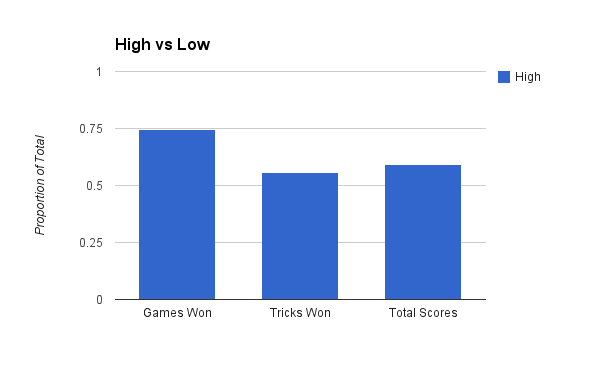
\includegraphics[width=\textwidth]{data/low.png}
        \caption{Results of the Low agent against the High agent.}
        \label{fig:results_low}
    \end{subfigure}
    \begin{subfigure}[b]{0.5\textwidth}
        \centering
        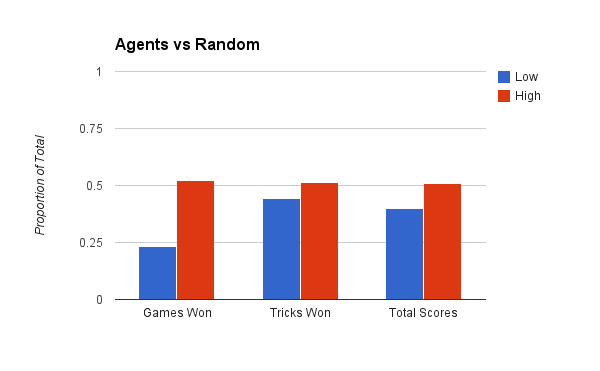
\includegraphics[width=\textwidth]{data/random.png}
        \caption{Results of the Random agent against other agents.}
        \label{fig:results_random}
    \end{subfigure}
    \caption{Results for the simple agents against each other.}
\end{figure}

\subsection{More Complex Strategies}

Figure \ref{fig:results_highlow} show the results for the HighLow agent against the simple strategies. The results show a staggering
favour for the HighLow agent, able to win handily against any of the simple strategies. This is not surprising, as the HighLow strategy
is generally decent enough play in human play. It tries to maximize the number of tricks each card can win, which leads it to be
a much stronger strategy than the simple three.

Figure \ref{fig:results_coophighlow} show the results for the CoopHighLow agent against the other strategies. Following the trend of 
the HighLow agent, the CoopHighLow proves to be very powerful compared to the simple strategies. This also shows the results of an
important competition. The CoopHighLow and HighLow agents both prove strong agents, but only one of the tries to cooperate with
their team mate. The results favour the CoopHighLow agent, who took on average about a point more per game.

\begin{figure}[ht]
    \begin{subfigure}[b]{0.5\textwidth}
        \centering
        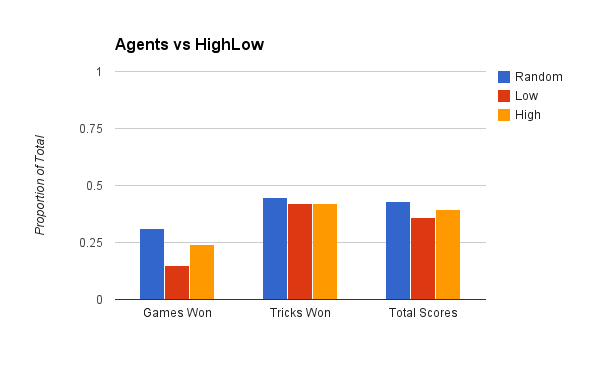
\includegraphics[width=\textwidth]{data/highlow.png}
        \caption{Results of the HighLow agent against other agents.}
        \label{fig:results_highlow}
    \end{subfigure}
    \begin{subfigure}[b]{0.5\textwidth}
        \centering
        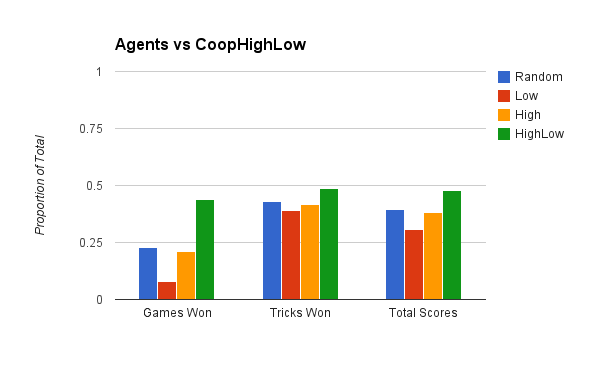
\includegraphics[width=\textwidth]{data/coophighlow.png}
        \caption{Results of the CoopHighLow agent against other agents.}
        \label{fig:results_coophighlow}
    \end{subfigure}
    \caption{Results for the two HighLow family strategies.}
\end{figure}


\subsection{Markov Decision Strategy}

Here, we show the results of two different Markov agents. They follow the same strategy, however the values they assign to each card
is different. The first agent uses the number of tricks a card wins out of all possible tricks given the current trump suit as the value for
each card. This proved to perform strangely, so an additional value base was formed. Markov2 uses a very similar value base; the value of
a card is the number of tricks the card can win which derive from the current trick and given the trump suit. This different value
base lends itself more closely to the actual values of the cards. For example, an ace that isn't the lead suit or trump cannot win any tricks,
so it should not be considered a powerful card. When leading a trick, Markov2 behaves identically to Markov. Both Markov agents used a threshold
$\tau=0.25$ due to there being 4 players in the game.

Something worth mentioning, these Markov strategies precomputed all the values of the cards and stored them for quick lookup when needed during
the games. They perform much faster this way, but used quite a bit of memory (around 1GB). However, the time taken to precompute the values
was only on the order of a second or two, so in real games they can be calculated on the fly quickly enough, human players would not notice
a considerable delay.

As mentioned, Markov performs strangely. Markov proves worse than Random, but slightly better than both Low and High. This is strange due to
the results shown in Figure \ref{fig:results_random}, showing that High is better than Random. When played against HighLow and CoopHighLow, Markov
did not do well at all, losing most of the games and averaging relatively low scores.

The Markov2 agent shows more promise than the Markov agent, showing it is actually slightly better than Random and still better
than both High and Low. Markov2 also is quite a bit better than the Markov agent.

This high that Markov2 experienced is quickly brought down by the soul crushing HighLow and CoopHighLow agents. Although Markov2
performed much better than Markov against these two agents, Markov2 was still trounced. Rather unfortunate. These results solidify
the Markov agents on par with the simple strategies.

\begin{figure}[ht]
    \begin{subfigure}[b]{0.5\textwidth}
        \centering
        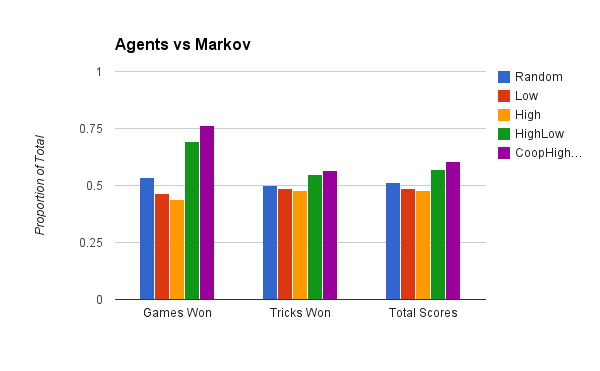
\includegraphics[width=\textwidth]{data/markov.png}
        \caption{Results of the Markov agent against other agents.}
        \label{fig:results_markov}
    \end{subfigure}
    \begin{subfigure}[b]{0.5\textwidth}
        \centering
        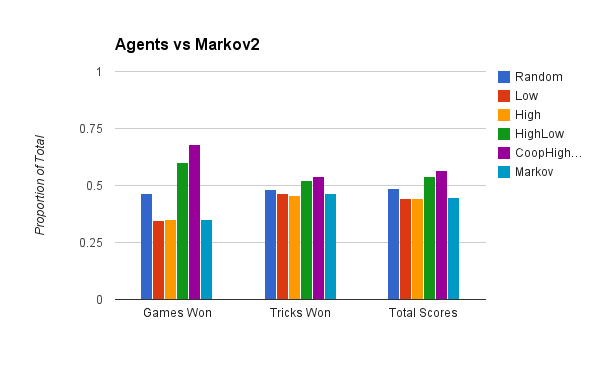
\includegraphics[width=\textwidth]{data/markov2.png}
        \caption{Results of the Markov2 agent against other agents.}
        \label{fig:results_markov2}
    \end{subfigure}
    \caption{Results for the two Markov family strategies.}
\end{figure}


\subsection{Card Counting Strategy}

The CardCounting was modelling off of how I personally play euchre, for the most part. Human players tend to keep track of what suit
players hold and play accordingly, and play differently depending on how many cards are in the trick. The CardCounting, similar to the
HighLow agent, performs very well against the simple strategies. The results are promising, as the agent achieves very high average
scores in each game.

Surprisingly, the more complex strategy modelled after more human play performs not as well as expected against the relatively simple
CoopHighLow agent. CardCounting was able to beat the HighLow agent. However, against the CoopHighLow agent, the CardCounting
essentially tied, performing slightly worse but taking more tricks. It is due to this disappointing result that the Hybrid strategy
was created, in hopes to beat the CoopHighLow agent.

As shown in the previous subsection, the Markov agents are not very powerful. They are swept aside by the CardCounting agent.

\begin{figure}[ht]
    \centering
    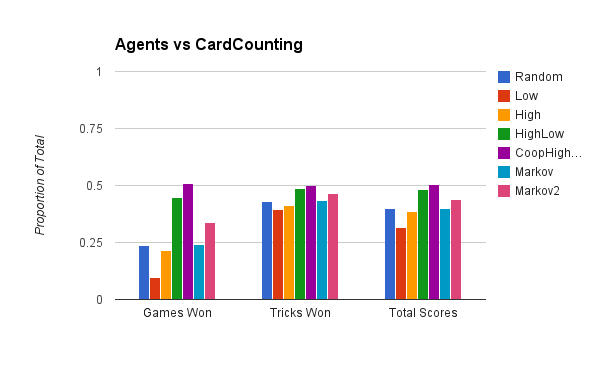
\includegraphics[scale=0.5]{data/cardcounting.png}
    \caption{Results of the CardCounting agent against other agents.}
    \label{fig:results_cardcounting}
\end{figure}


\subsection{Hybrid Strategy}

The Hybrid strategy was born out of the disappointing results of the CardCounting agent. A weakness of the CardCounting agent is that
it tends to play relatively passively, leading with low cards or generally playing Low too often. The Hybrid strategy used the Markov
decision process in order to determine which of the CardCounting and CoopHighLow strategies to play. When the hand was strong, a CoopHighLow
strategy was played, and CardCounting otherwise. The Hybrid agent uses the same card values as the Markov agent. After seeing the improvement
of Markov2 over Markov, a Hybrid2 agent was created as well in hopes of seeing the same type of improvement. Both Hybrid agents used
a threshold $\tau=0.25$ again, same as with the Markov agents.

Figure \ref{fig:results_hybrid} shows the results of the Hybrid agent against the other agents. Again, the wrath of the CoopHighLow agent
is seen, the Hybrid agent essentially equivalent to the CoopHighLow agent. Hybrid, however, does prove a slight improvement over the CardCounting
agent.

Figure \ref{fig:results_hybrid} shows the results of the Hybrid2 agent against the other agents. After seeing the improvement of the Markov2
agent over the Markov agent, it was hoped that Hybrid2 would see a similar improvement over Hybrid. Strangely, Hybrid2 tended to perform slightly
worse than Hybrid overall, losing to Hybrid in addition to losing to the CoopHighLow agent.

\begin{figure}[ht]
    \begin{subfigure}[b]{0.5\textwidth}
        \centering
        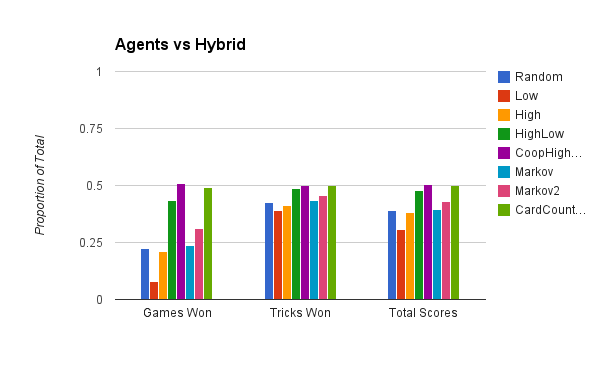
\includegraphics[width=\textwidth]{data/hybrid.png}
    \caption{Results of the Hybrid agent against other agents.}
    \label{fig:results_hybrid}
    \end{subfigure}
    \begin{subfigure}[b]{0.5\textwidth}
        \centering
        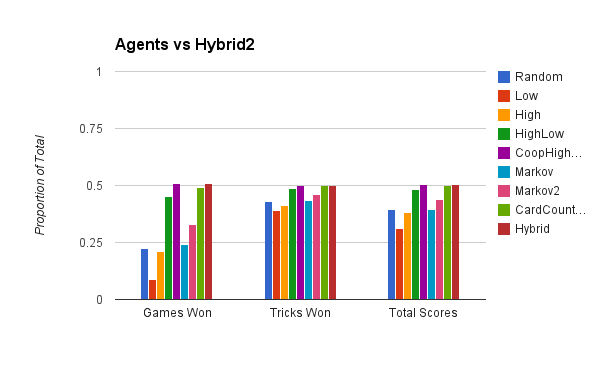
\includegraphics[width=\textwidth]{data/hybrid2.png}
    \caption{Results of the Hybrid2 agent against other agents.}
    \label{fig:results_hybrid2}
    \end{subfigure}
    \caption{Results for the two Hybrid family strategies.}
\end{figure}



\subsection{Monte Carlo Agent}

The MonteCarlo agent seems to be the only agent capable of toppling the CoopHighLow agent. Two different time limits were given to the MonteCarlo agent,
MonteCarlo10 was given 10 seconds for each decision and MonteCarlo60 was given 60 seconds. Due to the amount of time the MonteCarlo agents took,
fewer games were played and only against the strongest other agent, CoopHighLow. MonteCarlo10 played 31 games against CoopHighLow, while MonteCarlo60
only played 5. More games would be required for a stronger conclusion, however due to time constraints, this was not possible.

Figure \ref{fig:results_montecarlo} shows the results of the two MonteCarlo agents against CoopHighLow. MonteCarlo10 notably does poorly. This
is likely due to not being able to search enough of the game tree before being forced to make a decision. At the beginning of the game, only
a few hundred runs were able to complete. Not enough information could be gathered in order to make a good decision, as there are
$5 {18 \choose 5}{13 \choose 5}{8 \choose 5} \approx 3 \cdot 10^9$ possible branches to traverse at the start of the game -- not including
playing out each branch.

Given much more time, the MonteCarlo60 agent was able to beat the CoopHighLow agent. However, given a minute per decision makes for a very slow
game of euchre, so this is not a great outcome. Additionally, the results are still not wholly conclusive as not enough trials could be performed. 

\begin{figure}[ht]
    \centering
    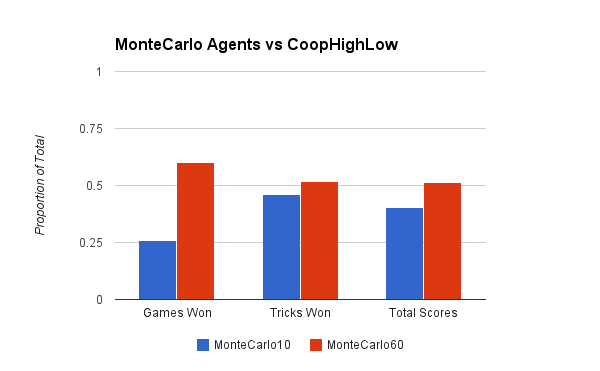
\includegraphics[scale=0.5]{data/montecarlo.png}
    \caption{Results of the two MonteCarlo agents against CoopHighLow.}
    \label{fig:results_montecarlo}
\end{figure}

\subsection{Mixed Agent Teams}

In addition to the above tests, mixed agent teams were also studied. These tests were ideally performed to view which agents were powerful cooperators.
Unfortunately, all the results were, simply put, rather boring. No mixed agent team was able to beat a team of CoopHighLow agents consistently.
Other games ended up as expected. So, to save the reader from many more charts, these results are omitted.

